\documentclass[letterpaper,12pt,fleqn]{article}
\usepackage{matharticle}
\usepackage{tikz}
\pagestyle{empty}
\renewcommand{\o}{\theta}
\newcommand{\w}{\omega}
\newcommand{\Arg}[1]{\mathrm{Arg}\,#1}
\begin{document}
\section*{Roots}
\begin{definition}
Let $z_1=r_1e^{i\o_1}$ and $z_2=r_2e^{i\o_2}$. To say that $z_1=z_2$ means:
\begin{enumerate}
\item $r_1=r_2$
\item $\o_1=\o_2+2\pi k, k\in\Z$
\end{enumerate}
\end{definition}

\begin{theorem}
The equation $z^n=z_0$ has $n$ roots all placed on the circle with center at $0$
and radius $\sqrt[n]{\abs{z_0}}$, starting at $\frac{\o_0}{n}$ and evenly spaced
by $\frac{2\pi}{n}$.
\end{theorem}

\begin{theproof}
Let $z=re^{i\o}$ and $z_0=r_0e^{1\o_0}$.
\begin{eqnarray*}
z^n &=& z_0 \\
\left(re^{i\o}\right)^n &=& r_0e^{1\o_0} \\
r^ne^{i(n\o)} &=& r_0e^{i\o_0} \\
r^n=r_0 &\mbox{and}& n\o=\o_0+2\pi k \\
r=\sqrt[n]{r_0} &\mbox{and}& \o=\frac{\o_0}{n}+k\frac{2\pi}{n} \\
\end{eqnarray*}
Note that unique roots are obtained for $0\le k<n$.
\end{theproof}

\begin{definition}
The $n^{th}$ roots of $z=re^{i\o}$, denoted $c_k$, are given by:
\[c_k=\sqrt[n]{r}e^{i(\frac{\o}{n}+\frac{2\pi k}{n})}\]
To say that $c_0$ is the \emph{principle root} means $\o=\Arg{z}$.
\end{definition}

Let $\w_n=e^{i\frac{2\pi}{n}}$.
\[\w_n^k=e^{i\frac{2\pi k}{n}}\]
\[c_k=\sqrt[n]{r}e^{i(\frac{\o}{n}+\frac{2\pi k}{n})}=
    \sqrt[n]{r}e^{i(\frac{\o}{n})}e^{i(\frac{2\pi k}{n})}=
    c_0\w_n^k\]
\newpage
\begin{example}
Find the fourth roots of $1$.

\begin{minipage}{3in}
\begin{eqnarray*}
z^4 &=& 1 \\
z^4 &=& e^{i(0+2\pi k)} \\
z &=& \left[e^{i(2\pi k)}\right]^{\frac{1}{4}} \\
z &=& e^{i(k\frac{\pi}{2})}, k=0,1,2,3 \\
z &=& 1,i,-1,-i \\
\w &=& e^{i\frac{2\pi}{4}}=e^{i\frac{\pi}{2}}=i \\
c_0 &=& 1 \\
c_1 &=& c_0\cdot i=1\cdot i=i \\
c_2 &=& c_1\cdot i=i\cdot i=-1 \\
c_3 &=& c_2\cdot i=-1\cdot i=-i \\
\end{eqnarray*}
\end{minipage}
\begin{minipage}{3in}
\begin{tikzpicture}
\draw (-3,0) -- (3,0);
\draw (0,-3) -- (0,3);
\draw (0,0) circle [radius=2];
\draw [fill=black] (2,0) circle [radius=0.05];
\draw [fill=black] (0,2) circle [radius=0.05];
\draw [fill=black] (-2,0) circle [radius=0.05];
\draw [fill=black] (0,-2) circle [radius=0.05];
\draw [dashed] (2,0) -- (0,2) -- (-2,0) -- (0,-2) -- (2,0);
\node [below right] at (2,0) {$1$};
\node [above right] at (0,2) {$i$};
\node [above left] at (-2,0) {$-1$};
\node [below left] at (0,-2) {$-i$};
\end{tikzpicture}
\end{minipage}
\end{example}

\begin{example}
Find the cubed roots of $i$.

\begin{minipage}{3in}
\begin{eqnarray*}
z^3 &=& i \\
z^3 &=& e^{i(\frac{\pi}{2}+2\pi k)} \\
z &=& \left[e^{i(\frac{\pi}{2}+2\pi k)}\right]^{\frac{1}{3}} \\
z &=& e^{i(\frac{\pi}{6}+\frac{2}{3}\pi k)}, k=0,1,2 \\
z &=& e^{i\frac{\pi}{6}}, e^{i\frac{5\pi}{6}}, e^{i\frac{9\pi}{6}}=e^{i\frac{3\pi}{2}}=-i\\
\w &=& e^{i\frac{2\pi}{3}} \\
c_0 &=& e^{i\frac{\pi}{6}} \\
c_1 &=& e^{i\frac{\pi}{6}}e^{i\frac{2\pi}{3}}=e^{i\frac{5\pi}{6}} \\
c_2 &=& e^{i\frac{5\pi}{6}}e^{i\frac{2\pi}{3}}=e^{i\frac{3\pi}{2}}=-i \\
\end{eqnarray*}
\end{minipage}
\begin{minipage}{3in}
\begin{tikzpicture}
\draw (-3,0) -- (3,0);
\draw (0,-3) -- (0,3);
\draw (0,0) circle [radius=2];
\draw [fill=black] (1.732,1) circle [radius=0.05];
\draw [fill=black] (-1.732,1) circle [radius=0.05];
\draw [fill=black] (0,-2) circle [radius=0.05];
\draw [dashed] (1.732,1) -- (-1.732,1) -- (0,-2) -- (1.732,1);
\node [above right] at (1.732,1) {$c_0$};
\node [above left] at (-1.732,1) {$c_1$};
\node [below right] at (0,-2) {$c_2$};
\end{tikzpicture}
\end{minipage}
\end{example}

Note that the roots are the vertices of an $n$-regular polygon.

\begin{theorem}
  $\forall\,z\in\C$:
  \[z^n-1=\prod_{k=0}^{n-1}{\left(1-e^{i\frac{2\pi k}{n}}\right)}\]
\end{theorem}

\begin{theproof}
  Assume $z\in\C$ \\
  The roots of $z^n-1=0$ are the $n^{th}$ roots of unity:
  \[z=e^{i\frac{2\pi k}{n}},\hspace{0.25in}0\le k<n\]
  \[\therefore z^n-1=\prod_{k=0}^{n-1}{\left(1-e^{i\frac{2\pi k}{n}}\right)}\]
\end{theproof}

\begin{corollary}
  $\forall\,n\in\N$:
  \[\prod_{k=1}^{n-1}{\abs{1-e^{i\frac{2\pi k}{n}}}}=n\]
\end{corollary}

\begin{theproof}
  Assume $n\in\N$
  \[z^n-1=\prod_{k=0}^{n-1}{\left(1-e^{i\frac{2\pi k}{n}}\right)}=
  (z-1)\prod_{k=1}^{n-1}{\left(1-e^{i\frac{2\pi k}{n}}\right)}\]
  Assume $z\ne1$
  \[\frac{z^n-1}{z-1}=\prod_{k=1}^{n-1}{\left(1-e^{i\frac{2\pi k}{n}}\right)}\]
  \[\abs{\frac{z^n-1}{z-1}}=\abs{\prod_{k=1}^{n-1}
    {\left(1-e^{i\frac{2\pi k}{n}}\right)}}=
  \prod_{k=1}^{n-1}{\abs{1-e^{i\frac{2\pi k}{n}}}}\]
  Let $z\to1$
  \begin{eqnarray*}
    \lim_{z\to1}{\abs{\frac{z^n-1}{z-1}}} &=&
    \abs{\lim_{z\to1}{\frac{z^n-1}{z-1}}} \\
    &=& \abs{\lim_{z\to1}{\frac{nz^{n-1}}{1}}}\hspace{0.25in}
    \mbox{(L'Hospital)} \\
    &=& \abs{n} \\
    &=& n \\
  \end{eqnarray*}
  \[\therefore\prod_{k=1}^{n-1}{\abs{1-e^{i\frac{2\pi k}{n}}}}=n\]
\end{theproof}
\newpage
Geometrically, this is the product of the line segments from $1$ to each of the
other $n-1$ roots. For example, for $n=8$:

\begin{figure}[h]
  \setlength{\leftskip}{1in}
  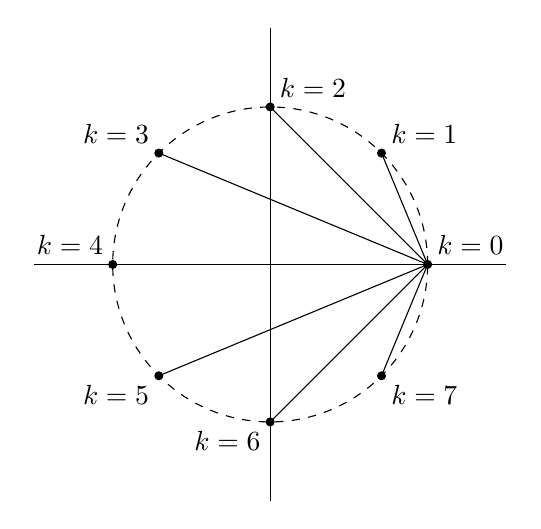
\begin{tikzpicture}
    \draw (-3,0) -- (3,0);
    \draw (0,-3) -- (0,3);
    \draw [dashed] (0,0) circle [radius=2];
    \draw [fill=black] (2,0) circle [radius=0.05];
    \draw [fill=black] ({sqrt(2)},{sqrt(2)}) circle [radius=0.05];
    \draw [fill=black] (0,2) circle [radius=0.05];
    \draw [fill=black] ({-sqrt(2)},{sqrt(2)}) circle [radius=0.05];
    \draw [fill=black] (-2,0) circle [radius=0.05];
    \draw [fill=black] ({-sqrt(2)},{-sqrt(2)}) circle [radius=0.05];
    \draw [fill=black] (0,-2) circle [radius=0.05];
    \draw [fill=black] ({sqrt(2)},{-sqrt(2)}) circle [radius=0.05];
    \draw (2,0) -- ({sqrt(2)},{sqrt(2)});
    \draw (2,0) -- (0,2);
    \draw (2,0) -- (-{sqrt(2)},{sqrt(2)});
    \draw (2,0) -- (-2,0);
    \draw (2,0) -- (-{sqrt(2)},{-sqrt(2)});
    \draw (2,0) -- (0,-2);
    \draw (2,0) -- ({sqrt(2)},{-sqrt(2)});
    \node [above right] at (2,0) {$k=0$};
    \node [above right] at ({sqrt(2)},{sqrt(2)}) {$k=1$};
    \node [above right] at (0,2) {$k=2$};
    \node [above left] at ({-sqrt(2)},{sqrt(2)}) {$k=3$};
    \node [above left] at (-2,0) {$k=4$};
    \node [below left] at ({-sqrt(2)},{-sqrt(2)}) {$k=5$};
    \node [below left] at (0,-2) {$k=6$};
    \node [below right] at ({sqrt(2)},{-sqrt(2)}) {$k=7$};
  \end{tikzpicture}
\end{figure}

\begin{corollary}
  $\forall\,n\in\N$:
  \[2^{n-1}\prod_{k=1}^{n-1}{\sin{\frac{k\pi}{n}}}=n\]
\end{corollary}

\begin{theproof}
  Assume $n\in\N$
  \begin{eqnarray*}
    \prod_{k=1}^{n-1}{\abs{1-e^{i\frac{2\pi k}{n}}}} &=& n \\
    \prod_{k=1}^{n-1}{
    \abs{e^{i\frac{k\pi}{n}}}\abs{e^{-\frac{k\pi}{n}}-e^{i\frac{\pi k}{n}}}} &=& n \\
    \prod_{k=1}^{n-1}{(1)\abs{2i\sin{\frac{k\pi}{n}}}} &=& n \\
    2^{n-1}\prod_{k=1}^{n-1}{\abs{\sin{\frac{k\pi}{n}}}} &=& n \\
  \end{eqnarray*}
  But $0<\frac{k\pi}{n}<\pi$ for $0<k<n$, so only in QI and QII
  \[\therefore2^{n-1}\prod_{k=1}^{n-1}{\sin{\frac{k\pi}{n}}}=n\]
\end{theproof}

\end{document}
